% Created by tikzDevice version 0.12.3 on 2020-01-31 10:30:04
% !TEX encoding = UTF-8 Unicode
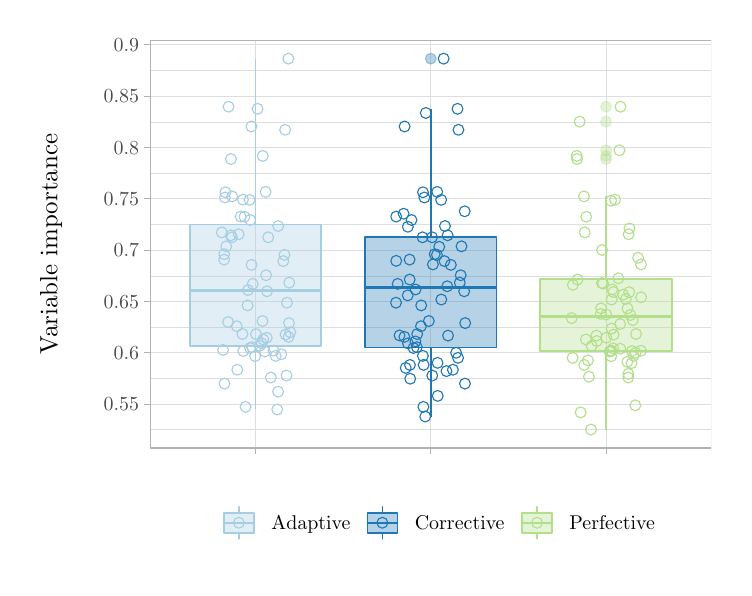
\begin{tikzpicture}[x=1pt,y=1pt]
\definecolor{fillColor}{RGB}{255,255,255}
\path[use as bounding box,fill=fillColor,fill opacity=0.00] (0,0) rectangle (251.50,195.13);
\begin{scope}
\path[clip] (  0.00,  0.00) rectangle (251.50,195.13);
\definecolor{drawColor}{RGB}{255,255,255}
\definecolor{fillColor}{RGB}{255,255,255}

\path[draw=drawColor,line width= 0.5pt,line join=round,line cap=round,fill=fillColor] (  0.00,  0.00) rectangle (251.50,195.13);
\end{scope}
\begin{scope}
\path[clip] ( 44.29, 43.20) rectangle (247.00,190.63);
\definecolor{fillColor}{RGB}{255,255,255}

\path[fill=fillColor] ( 44.29, 43.20) rectangle (247.00,190.63);
\definecolor{drawColor}{gray}{0.87}

\path[draw=drawColor,line width= 0.1pt,line join=round] ( 44.29, 49.88) --
	(247.00, 49.88);

\path[draw=drawColor,line width= 0.1pt,line join=round] ( 44.29, 68.43) --
	(247.00, 68.43);

\path[draw=drawColor,line width= 0.1pt,line join=round] ( 44.29, 86.97) --
	(247.00, 86.97);

\path[draw=drawColor,line width= 0.1pt,line join=round] ( 44.29,105.52) --
	(247.00,105.52);

\path[draw=drawColor,line width= 0.1pt,line join=round] ( 44.29,124.06) --
	(247.00,124.06);

\path[draw=drawColor,line width= 0.1pt,line join=round] ( 44.29,142.61) --
	(247.00,142.61);

\path[draw=drawColor,line width= 0.1pt,line join=round] ( 44.29,161.15) --
	(247.00,161.15);

\path[draw=drawColor,line width= 0.1pt,line join=round] ( 44.29,179.70) --
	(247.00,179.70);

\path[draw=drawColor,line width= 0.2pt,line join=round] ( 44.29, 59.15) --
	(247.00, 59.15);

\path[draw=drawColor,line width= 0.2pt,line join=round] ( 44.29, 77.70) --
	(247.00, 77.70);

\path[draw=drawColor,line width= 0.2pt,line join=round] ( 44.29, 96.24) --
	(247.00, 96.24);

\path[draw=drawColor,line width= 0.2pt,line join=round] ( 44.29,114.79) --
	(247.00,114.79);

\path[draw=drawColor,line width= 0.2pt,line join=round] ( 44.29,133.33) --
	(247.00,133.33);

\path[draw=drawColor,line width= 0.2pt,line join=round] ( 44.29,151.88) --
	(247.00,151.88);

\path[draw=drawColor,line width= 0.2pt,line join=round] ( 44.29,170.42) --
	(247.00,170.42);

\path[draw=drawColor,line width= 0.2pt,line join=round] ( 44.29,188.97) --
	(247.00,188.97);

\path[draw=drawColor,line width= 0.2pt,line join=round] ( 82.30, 43.20) --
	( 82.30,190.63);

\path[draw=drawColor,line width= 0.2pt,line join=round] (145.65, 43.20) --
	(145.65,190.63);

\path[draw=drawColor,line width= 0.2pt,line join=round] (208.99, 43.20) --
	(208.99,190.63);
\definecolor{drawColor}{RGB}{166,206,227}

\path[draw=drawColor,line width= 0.6pt,line join=round] ( 82.30,123.99) -- ( 82.30,183.93);

\path[draw=drawColor,line width= 0.6pt,line join=round] ( 82.30, 80.02) -- ( 82.30, 57.16);
\definecolor{fillColor}{RGB}{166,206,227}

\path[draw=drawColor,line width= 0.6pt,line join=round,line cap=round,fill=fillColor,fill opacity=0.33] ( 58.55,123.99) --
	( 58.55, 80.02) --
	(106.06, 80.02) --
	(106.06,123.99) --
	( 58.55,123.99) --
	cycle;

\path[draw=drawColor,line width= 1.1pt,line join=round] ( 58.55,100.09) -- (106.06,100.09);
\definecolor{drawColor}{RGB}{31,120,180}
\definecolor{fillColor}{RGB}{31,120,180}

\path[draw=drawColor,draw opacity=0.33,line width= 0.4pt,line join=round,line cap=round,fill=fillColor,fill opacity=0.33] (145.65,183.93) circle (  1.96);
\definecolor{drawColor}{RGB}{31,120,180}

\path[draw=drawColor,line width= 0.6pt,line join=round] (145.65,119.56) -- (145.65,165.80);

\path[draw=drawColor,line width= 0.6pt,line join=round] (145.65, 79.61) -- (145.65, 54.61);

\path[draw=drawColor,line width= 0.6pt,line join=round,line cap=round,fill=fillColor,fill opacity=0.33] (121.89,119.56) --
	(121.89, 79.61) --
	(169.40, 79.61) --
	(169.40,119.56) --
	(121.89,119.56) --
	cycle;

\path[draw=drawColor,line width= 1.1pt,line join=round] (121.89,101.11) -- (169.40,101.11);
\definecolor{drawColor}{RGB}{178,223,138}
\definecolor{fillColor}{RGB}{178,223,138}

\path[draw=drawColor,draw opacity=0.33,line width= 0.4pt,line join=round,line cap=round,fill=fillColor,fill opacity=0.33] (208.99,166.55) circle (  1.96);

\path[draw=drawColor,draw opacity=0.33,line width= 0.4pt,line join=round,line cap=round,fill=fillColor,fill opacity=0.33] (208.99,147.65) circle (  1.96);

\path[draw=drawColor,draw opacity=0.33,line width= 0.4pt,line join=round,line cap=round,fill=fillColor,fill opacity=0.33] (208.99,161.17) circle (  1.96);

\path[draw=drawColor,draw opacity=0.33,line width= 0.4pt,line join=round,line cap=round,fill=fillColor,fill opacity=0.33] (208.99,148.79) circle (  1.96);

\path[draw=drawColor,draw opacity=0.33,line width= 0.4pt,line join=round,line cap=round,fill=fillColor,fill opacity=0.33] (208.99,150.83) circle (  1.96);
\definecolor{drawColor}{RGB}{178,223,138}

\path[draw=drawColor,line width= 0.6pt,line join=round] (208.99,104.23) -- (208.99,134.16);

\path[draw=drawColor,line width= 0.6pt,line join=round] (208.99, 78.27) -- (208.99, 49.90);

\path[draw=drawColor,line width= 0.6pt,line join=round,line cap=round,fill=fillColor,fill opacity=0.33] (185.24,104.23) --
	(185.24, 78.27) --
	(232.75, 78.27) --
	(232.75,104.23) --
	(185.24,104.23) --
	cycle;

\path[draw=drawColor,line width= 1.1pt,line join=round] (185.24, 90.74) -- (232.75, 90.74);
\definecolor{drawColor}{RGB}{166,206,227}

\path[draw=drawColor,line width= 0.4pt,line join=round,line cap=round] ( 85.72, 78.09) circle (  1.96);

\path[draw=drawColor,line width= 0.4pt,line join=round,line cap=round] ( 72.58,166.55) circle (  1.96);

\path[draw=drawColor,line width= 0.4pt,line join=round,line cap=round] ( 75.75, 71.52) circle (  1.96);

\path[draw=drawColor,line width= 0.4pt,line join=round,line cap=round] ( 73.46,147.65) circle (  1.96);

\path[draw=drawColor,line width= 0.4pt,line join=round,line cap=round] ( 84.85, 89.13) circle (  1.96);

\path[draw=drawColor,line width= 0.4pt,line join=round,line cap=round] ( 77.79,132.98) circle (  1.96);

\path[draw=drawColor,line width= 0.4pt,line join=round,line cap=round] ( 70.98,111.32) circle (  1.96);

\path[draw=drawColor,line width= 0.4pt,line join=round,line cap=round] ( 82.49, 84.41) circle (  1.96);

\path[draw=drawColor,line width= 0.4pt,line join=round,line cap=round] ( 85.14, 82.47) circle (  1.96);

\path[draw=drawColor,line width= 0.4pt,line join=round,line cap=round] ( 77.60, 84.44) circle (  1.96);
\definecolor{drawColor}{RGB}{31,120,180}

\path[draw=drawColor,line width= 0.4pt,line join=round,line cap=round] (138.23, 68.28) circle (  1.96);

\path[draw=drawColor,line width= 0.4pt,line join=round,line cap=round] (143.86,164.31) circle (  1.96);

\path[draw=drawColor,line width= 0.4pt,line join=round,line cap=round] (153.65, 71.52) circle (  1.96);

\path[draw=drawColor,line width= 0.4pt,line join=round,line cap=round] (133.17,110.87) circle (  1.96);

\path[draw=drawColor,line width= 0.4pt,line join=round,line cap=round] (144.95, 89.13) circle (  1.96);

\path[draw=drawColor,line width= 0.4pt,line join=round,line cap=round] (157.92,128.77) circle (  1.96);

\path[draw=drawColor,line width= 0.4pt,line join=round,line cap=round] (138.00,111.32) circle (  1.96);

\path[draw=drawColor,line width= 0.4pt,line join=round,line cap=round] (140.75, 84.41) circle (  1.96);

\path[draw=drawColor,line width= 0.4pt,line join=round,line cap=round] (140.11, 81.74) circle (  1.96);

\path[draw=drawColor,line width= 0.4pt,line join=round,line cap=round] (148.11, 74.02) circle (  1.96);
\definecolor{drawColor}{RGB}{178,223,138}

\path[draw=drawColor,line width= 0.4pt,line join=round,line cap=round] (210.28, 78.09) circle (  1.96);

\path[draw=drawColor,line width= 0.4pt,line join=round,line cap=round] (214.20,166.55) circle (  1.96);

\path[draw=drawColor,line width= 0.4pt,line join=round,line cap=round] (217.03, 68.71) circle (  1.96);

\path[draw=drawColor,line width= 0.4pt,line join=round,line cap=round] (198.53,147.65) circle (  1.96);

\path[draw=drawColor,line width= 0.4pt,line join=round,line cap=round] (214.13, 79.10) circle (  1.96);

\path[draw=drawColor,line width= 0.4pt,line join=round,line cap=round] (212.25,132.98) circle (  1.96);

\path[draw=drawColor,line width= 0.4pt,line join=round,line cap=round] (207.48,102.87) circle (  1.96);

\path[draw=drawColor,line width= 0.4pt,line join=round,line cap=round] (211.55, 79.24) circle (  1.96);

\path[draw=drawColor,line width= 0.4pt,line join=round,line cap=round] (201.71, 82.47) circle (  1.96);

\path[draw=drawColor,line width= 0.4pt,line join=round,line cap=round] (219.83, 84.44) circle (  1.96);
\definecolor{drawColor}{RGB}{166,206,227}

\path[draw=drawColor,line width= 0.4pt,line join=round,line cap=round] ( 77.89, 78.28) circle (  1.96);

\path[draw=drawColor,line width= 0.4pt,line join=round,line cap=round] ( 83.08,165.80) circle (  1.96);

\path[draw=drawColor,line width= 0.4pt,line join=round,line cap=round] ( 84.95,148.79) circle (  1.96);

\path[draw=drawColor,line width= 0.4pt,line join=round,line cap=round] ( 94.43, 88.38) circle (  1.96);

\path[draw=drawColor,line width= 0.4pt,line join=round,line cap=round] ( 73.89,134.16) circle (  1.96);

\path[draw=drawColor,line width= 0.4pt,line join=round,line cap=round] ( 92.36,110.78) circle (  1.96);

\path[draw=drawColor,line width= 0.4pt,line join=round,line cap=round] ( 94.28, 83.40) circle (  1.96);

\path[draw=drawColor,line width= 0.4pt,line join=round,line cap=round] ( 93.18, 84.21) circle (  1.96);

\path[draw=drawColor,line width= 0.4pt,line join=round,line cap=round] ( 86.37, 83.09) circle (  1.96);
\definecolor{drawColor}{RGB}{31,120,180}

\path[draw=drawColor,line width= 0.4pt,line join=round,line cap=round] (143.08, 73.28) circle (  1.96);

\path[draw=drawColor,line width= 0.4pt,line join=round,line cap=round] (155.32,165.80) circle (  1.96);

\path[draw=drawColor,line width= 0.4pt,line join=round,line cap=round] (148.71,115.95) circle (  1.96);

\path[draw=drawColor,line width= 0.4pt,line join=round,line cap=round] (158.10, 88.38) circle (  1.96);

\path[draw=drawColor,line width= 0.4pt,line join=round,line cap=round] (135.85,127.90) circle (  1.96);

\path[draw=drawColor,line width= 0.4pt,line join=round,line cap=round] (150.60,110.78) circle (  1.96);

\path[draw=drawColor,line width= 0.4pt,line join=round,line cap=round] (136.12, 83.40) circle (  1.96);

\path[draw=drawColor,line width= 0.4pt,line join=round,line cap=round] (134.37, 83.92) circle (  1.96);

\path[draw=drawColor,line width= 0.4pt,line join=round,line cap=round] (136.60, 72.18) circle (  1.96);
\definecolor{drawColor}{RGB}{178,223,138}

\path[draw=drawColor,line width= 0.4pt,line join=round,line cap=round] (218.33, 78.27) circle (  1.96);

\path[draw=drawColor,line width= 0.4pt,line join=round,line cap=round] (199.48,161.17) circle (  1.96);

\path[draw=drawColor,line width= 0.4pt,line join=round,line cap=round] (198.41,148.79) circle (  1.96);

\path[draw=drawColor,line width= 0.4pt,line join=round,line cap=round] (210.65, 78.27) circle (  1.96);

\path[draw=drawColor,line width= 0.4pt,line join=round,line cap=round] (201.02,134.16) circle (  1.96);

\path[draw=drawColor,line width= 0.4pt,line join=round,line cap=round] (213.46,104.57) circle (  1.96);

\path[draw=drawColor,line width= 0.4pt,line join=round,line cap=round] (218.19, 73.89) circle (  1.96);

\path[draw=drawColor,line width= 0.4pt,line join=round,line cap=round] (211.72, 84.21) circle (  1.96);

\path[draw=drawColor,line width= 0.4pt,line join=round,line cap=round] (209.07, 83.09) circle (  1.96);
\definecolor{drawColor}{RGB}{166,206,227}

\path[draw=drawColor,line width= 0.4pt,line join=round,line cap=round] ( 79.47, 94.77) circle (  1.96);

\path[draw=drawColor,line width= 0.4pt,line join=round,line cap=round] ( 71.26,133.76) circle (  1.96);

\path[draw=drawColor,line width= 0.4pt,line join=round,line cap=round] ( 79.60,100.32) circle (  1.96);

\path[draw=drawColor,line width= 0.4pt,line join=round,line cap=round] ( 76.97,126.86) circle (  1.96);

\path[draw=drawColor,line width= 0.4pt,line join=round,line cap=round] ( 75.55, 87.25) circle (  1.96);

\path[draw=drawColor,line width= 0.4pt,line join=round,line cap=round] ( 71.01,113.29) circle (  1.96);

\path[draw=drawColor,line width= 0.4pt,line join=round,line cap=round] ( 81.33,102.54) circle (  1.96);

\path[draw=drawColor,line width= 0.4pt,line join=round,line cap=round] ( 84.54, 81.06) circle (  1.96);

\path[draw=drawColor,line width= 0.4pt,line join=round,line cap=round] ( 78.33,126.79) circle (  1.96);

\path[draw=drawColor,line width= 0.4pt,line join=round,line cap=round] ( 73.81,119.38) circle (  1.96);

\path[draw=drawColor,line width= 0.4pt,line join=round,line cap=round] ( 71.11, 66.51) circle (  1.96);
\definecolor{drawColor}{RGB}{31,120,180}

\path[draw=drawColor,line width= 0.4pt,line join=round,line cap=round] (142.20, 94.77) circle (  1.96);

\path[draw=drawColor,line width= 0.4pt,line join=round,line cap=round] (143.35,133.76) circle (  1.96);

\path[draw=drawColor,line width= 0.4pt,line join=round,line cap=round] (146.43,109.58) circle (  1.96);

\path[draw=drawColor,line width= 0.4pt,line join=round,line cap=round] (133.16,126.86) circle (  1.96);

\path[draw=drawColor,line width= 0.4pt,line join=round,line cap=round] (142.12, 87.25) circle (  1.96);

\path[draw=drawColor,line width= 0.4pt,line join=round,line cap=round] (147.06,113.29) circle (  1.96);

\path[draw=drawColor,line width= 0.4pt,line join=round,line cap=round] (133.70,102.54) circle (  1.96);

\path[draw=drawColor,line width= 0.4pt,line join=round,line cap=round] (137.41, 81.06) circle (  1.96);

\path[draw=drawColor,line width= 0.4pt,line join=round,line cap=round] (137.38,123.19) circle (  1.96);

\path[draw=drawColor,line width= 0.4pt,line join=round,line cap=round] (142.68,119.38) circle (  1.96);

\path[draw=drawColor,line width= 0.4pt,line join=round,line cap=round] (158.01, 66.51) circle (  1.96);
\definecolor{drawColor}{RGB}{178,223,138}

\path[draw=drawColor,line width= 0.4pt,line join=round,line cap=round] (218.98, 76.56) circle (  1.96);

\path[draw=drawColor,line width= 0.4pt,line join=round,line cap=round] (214.08, 88.02) circle (  1.96);

\path[draw=drawColor,line width= 0.4pt,line join=round,line cap=round] (221.63,109.58) circle (  1.96);

\path[draw=drawColor,line width= 0.4pt,line join=round,line cap=round] (220.60,111.97) circle (  1.96);

\path[draw=drawColor,line width= 0.4pt,line join=round,line cap=round] (202.81, 69.01) circle (  1.96);

\path[draw=drawColor,line width= 0.4pt,line join=round,line cap=round] (207.94,102.66) circle (  1.96);

\path[draw=drawColor,line width= 0.4pt,line join=round,line cap=round] (216.15, 97.09) circle (  1.96);

\path[draw=drawColor,line width= 0.4pt,line join=round,line cap=round] (216.70, 74.40) circle (  1.96);

\path[draw=drawColor,line width= 0.4pt,line join=round,line cap=round] (201.83,126.80) circle (  1.96);

\path[draw=drawColor,line width= 0.4pt,line join=round,line cap=round] (209.04, 91.48) circle (  1.96);

\path[draw=drawColor,line width= 0.4pt,line join=round,line cap=round] (199.81, 56.12) circle (  1.96);
\definecolor{drawColor}{RGB}{166,206,227}

\path[draw=drawColor,line width= 0.4pt,line join=round,line cap=round] ( 73.40,120.09) circle (  1.96);

\path[draw=drawColor,line width= 0.4pt,line join=round,line cap=round] ( 80.86,159.43) circle (  1.96);

\path[draw=drawColor,line width= 0.4pt,line join=round,line cap=round] ( 85.98,135.79) circle (  1.96);

\path[draw=drawColor,line width= 0.4pt,line join=round,line cap=round] ( 93.03,158.22) circle (  1.96);

\path[draw=drawColor,line width= 0.4pt,line join=round,line cap=round] ( 80.42,125.62) circle (  1.96);

\path[draw=drawColor,line width= 0.4pt,line join=round,line cap=round] ( 80.91,109.42) circle (  1.96);

\path[draw=drawColor,line width= 0.4pt,line join=round,line cap=round] ( 89.59, 76.54) circle (  1.96);

\path[draw=drawColor,line width= 0.4pt,line join=round,line cap=round] ( 86.50, 99.86) circle (  1.96);

\path[draw=drawColor,line width= 0.4pt,line join=round,line cap=round] ( 70.15,121.15) circle (  1.96);

\path[draw=drawColor,line width= 0.4pt,line join=round,line cap=round] ( 71.43,135.66) circle (  1.96);

\path[draw=drawColor,line width= 0.4pt,line join=round,line cap=round] ( 86.92,119.39) circle (  1.96);
\definecolor{drawColor}{RGB}{31,120,180}

\path[draw=drawColor,line width= 0.4pt,line join=round,line cap=round] (151.75,120.09) circle (  1.96);

\path[draw=drawColor,line width= 0.4pt,line join=round,line cap=round] (136.20,159.43) circle (  1.96);

\path[draw=drawColor,line width= 0.4pt,line join=round,line cap=round] (147.99,135.79) circle (  1.96);

\path[draw=drawColor,line width= 0.4pt,line join=round,line cap=round] (155.66,158.22) circle (  1.96);

\path[draw=drawColor,line width= 0.4pt,line join=round,line cap=round] (138.70,125.62) circle (  1.96);

\path[draw=drawColor,line width= 0.4pt,line join=round,line cap=round] (152.90,109.42) circle (  1.96);

\path[draw=drawColor,line width= 0.4pt,line join=round,line cap=round] (142.81, 76.54) circle (  1.96);

\path[draw=drawColor,line width= 0.4pt,line join=round,line cap=round] (157.73, 99.86) circle (  1.96);

\path[draw=drawColor,line width= 0.4pt,line join=round,line cap=round] (151.61,101.68) circle (  1.96);

\path[draw=drawColor,line width= 0.4pt,line join=round,line cap=round] (142.84,135.66) circle (  1.96);

\path[draw=drawColor,line width= 0.4pt,line join=round,line cap=round] (146.13,119.39) circle (  1.96);
\definecolor{drawColor}{RGB}{178,223,138}

\path[draw=drawColor,line width= 0.4pt,line join=round,line cap=round] (211.02, 86.40) circle (  1.96);

\path[draw=drawColor,line width= 0.4pt,line join=round,line cap=round] (217.46,122.58) circle (  1.96);

\path[draw=drawColor,line width= 0.4pt,line join=round,line cap=round] (221.65, 97.70) circle (  1.96);

\path[draw=drawColor,line width= 0.4pt,line join=round,line cap=round] (213.83,150.83) circle (  1.96);

\path[draw=drawColor,line width= 0.4pt,line join=round,line cap=round] (207.20, 93.71) circle (  1.96);

\path[draw=drawColor,line width= 0.4pt,line join=round,line cap=round] (215.14, 98.64) circle (  1.96);

\path[draw=drawColor,line width= 0.4pt,line join=round,line cap=round] (202.44, 74.89) circle (  1.96);

\path[draw=drawColor,line width= 0.4pt,line join=round,line cap=round] (196.58, 90.19) circle (  1.96);

\path[draw=drawColor,line width= 0.4pt,line join=round,line cap=round] (201.30,121.15) circle (  1.96);

\path[draw=drawColor,line width= 0.4pt,line join=round,line cap=round] (211.67, 99.61) circle (  1.96);

\path[draw=drawColor,line width= 0.4pt,line join=round,line cap=round] (207.57,114.79) circle (  1.96);
\definecolor{drawColor}{RGB}{166,206,227}

\path[draw=drawColor,line width= 0.4pt,line join=round,line cap=round] ( 94.91, 85.06) circle (  1.96);

\path[draw=drawColor,line width= 0.4pt,line join=round,line cap=round] ( 90.18, 57.16) circle (  1.96);

\path[draw=drawColor,line width= 0.4pt,line join=round,line cap=round] ( 71.75,116.12) circle (  1.96);

\path[draw=drawColor,line width= 0.4pt,line join=round,line cap=round] ( 90.51,123.45) circle (  1.96);

\path[draw=drawColor,line width= 0.4pt,line join=round,line cap=round] ( 76.25,120.47) circle (  1.96);

\path[draw=drawColor,line width= 0.4pt,line join=round,line cap=round] ( 90.48, 63.59) circle (  1.96);

\path[draw=drawColor,line width= 0.4pt,line join=round,line cap=round] ( 93.70, 95.75) circle (  1.96);

\path[draw=drawColor,line width= 0.4pt,line join=round,line cap=round] ( 87.88, 68.71) circle (  1.96);

\path[draw=drawColor,line width= 0.4pt,line join=round,line cap=round] ( 78.73, 58.11) circle (  1.96);

\path[draw=drawColor,line width= 0.4pt,line join=round,line cap=round] ( 70.62, 78.69) circle (  1.96);

\path[draw=drawColor,line width= 0.4pt,line join=round,line cap=round] ( 80.36, 79.38) circle (  1.96);
\definecolor{drawColor}{RGB}{31,120,180}

\path[draw=drawColor,line width= 0.4pt,line join=round,line cap=round] (140.15,100.53) circle (  1.96);

\path[draw=drawColor,line width= 0.4pt,line join=round,line cap=round] (155.51, 75.82) circle (  1.96);

\path[draw=drawColor,line width= 0.4pt,line join=round,line cap=round] (156.77,116.12) circle (  1.96);

\path[draw=drawColor,line width= 0.4pt,line join=round,line cap=round] (150.78,123.45) circle (  1.96);

\path[draw=drawColor,line width= 0.4pt,line join=round,line cap=round] (137.34, 98.40) circle (  1.96);

\path[draw=drawColor,line width= 0.4pt,line join=round,line cap=round] (151.90, 83.86) circle (  1.96);

\path[draw=drawColor,line width= 0.4pt,line join=round,line cap=round] (133.09, 95.75) circle (  1.96);

\path[draw=drawColor,line width= 0.4pt,line join=round,line cap=round] (138.13, 73.26) circle (  1.96);

\path[draw=drawColor,line width= 0.4pt,line join=round,line cap=round] (142.99, 58.11) circle (  1.96);

\path[draw=drawColor,line width= 0.4pt,line join=round,line cap=round] (138.04,104.12) circle (  1.96);

\path[draw=drawColor,line width= 0.4pt,line join=round,line cap=round] (139.41, 79.38) circle (  1.96);
\definecolor{drawColor}{RGB}{178,223,138}

\path[draw=drawColor,line width= 0.4pt,line join=round,line cap=round] (211.23,100.53) circle (  1.96);

\path[draw=drawColor,line width= 0.4pt,line join=round,line cap=round] (196.90, 75.82) circle (  1.96);

\path[draw=drawColor,line width= 0.4pt,line join=round,line cap=round] (207.07, 91.70) circle (  1.96);

\path[draw=drawColor,line width= 0.4pt,line join=round,line cap=round] (217.78, 91.30) circle (  1.96);

\path[draw=drawColor,line width= 0.4pt,line join=round,line cap=round] (217.13,120.47) circle (  1.96);

\path[draw=drawColor,line width= 0.4pt,line join=round,line cap=round] (205.50, 83.86) circle (  1.96);

\path[draw=drawColor,line width= 0.4pt,line join=round,line cap=round] (216.73, 93.69) circle (  1.96);

\path[draw=drawColor,line width= 0.4pt,line join=round,line cap=round] (201.11, 73.26) circle (  1.96);

\path[draw=drawColor,line width= 0.4pt,line join=round,line cap=round] (203.56, 49.90) circle (  1.96);

\path[draw=drawColor,line width= 0.4pt,line join=round,line cap=round] (198.69,104.12) circle (  1.96);

\path[draw=drawColor,line width= 0.4pt,line join=round,line cap=round] (217.02, 70.01) circle (  1.96);
\definecolor{drawColor}{RGB}{166,206,227}

\path[draw=drawColor,line width= 0.4pt,line join=round,line cap=round] ( 86.15,105.66) circle (  1.96);

\path[draw=drawColor,line width= 0.4pt,line join=round,line cap=round] ( 80.20,132.91) circle (  1.96);

\path[draw=drawColor,line width= 0.4pt,line join=round,line cap=round] ( 91.65, 77.14) circle (  1.96);

\path[draw=drawColor,line width= 0.4pt,line join=round,line cap=round] ( 94.51,102.99) circle (  1.96);

\path[draw=drawColor,line width= 0.4pt,line join=round,line cap=round] ( 94.19,183.93) circle (  1.96);

\path[draw=drawColor,line width= 0.4pt,line join=round,line cap=round] ( 92.78,113.04) circle (  1.96);

\path[draw=drawColor,line width= 0.4pt,line join=round,line cap=round] ( 93.53, 69.42) circle (  1.96);

\path[draw=drawColor,line width= 0.4pt,line join=round,line cap=round] ( 72.43, 88.76) circle (  1.96);

\path[draw=drawColor,line width= 0.4pt,line join=round,line cap=round] ( 83.85, 80.14) circle (  1.96);

\path[draw=drawColor,line width= 0.4pt,line join=round,line cap=round] ( 88.85, 78.40) circle (  1.96);

\path[draw=drawColor,line width= 0.4pt,line join=round,line cap=round] ( 81.10, 79.69) circle (  1.96);
\definecolor{drawColor}{RGB}{31,120,180}

\path[draw=drawColor,line width= 0.4pt,line join=round,line cap=round] (156.47,105.66) circle (  1.96);

\path[draw=drawColor,line width= 0.4pt,line join=round,line cap=round] (149.41,132.91) circle (  1.96);

\path[draw=drawColor,line width= 0.4pt,line join=round,line cap=round] (154.81, 77.65) circle (  1.96);

\path[draw=drawColor,line width= 0.4pt,line join=round,line cap=round] (156.14,102.99) circle (  1.96);

\path[draw=drawColor,line width= 0.4pt,line join=round,line cap=round] (150.30,183.93) circle (  1.96);

\path[draw=drawColor,line width= 0.4pt,line join=round,line cap=round] (147.88,113.04) circle (  1.96);

\path[draw=drawColor,line width= 0.4pt,line join=round,line cap=round] (146.19, 69.42) circle (  1.96);

\path[draw=drawColor,line width= 0.4pt,line join=round,line cap=round] (149.47, 96.89) circle (  1.96);

\path[draw=drawColor,line width= 0.4pt,line join=round,line cap=round] (151.33, 71.03) circle (  1.96);

\path[draw=drawColor,line width= 0.4pt,line join=round,line cap=round] (143.66, 54.61) circle (  1.96);

\path[draw=drawColor,line width= 0.4pt,line join=round,line cap=round] (140.62, 79.69) circle (  1.96);
\definecolor{drawColor}{RGB}{178,223,138}

\path[draw=drawColor,line width= 0.4pt,line join=round,line cap=round] (205.66, 81.88) circle (  1.96);

\path[draw=drawColor,line width= 0.4pt,line join=round,line cap=round] (217.33, 99.55) circle (  1.96);

\path[draw=drawColor,line width= 0.4pt,line join=round,line cap=round] (219.69, 77.65) circle (  1.96);

\path[draw=drawColor,line width= 0.4pt,line join=round,line cap=round] (218.64, 89.47) circle (  1.96);

\path[draw=drawColor,line width= 0.4pt,line join=round,line cap=round] (210.82,132.61) circle (  1.96);

\path[draw=drawColor,line width= 0.4pt,line join=round,line cap=round] (197.01,102.19) circle (  1.96);

\path[draw=drawColor,line width= 0.4pt,line join=round,line cap=round] (219.57, 58.67) circle (  1.96);

\path[draw=drawColor,line width= 0.4pt,line join=round,line cap=round] (211.02, 96.89) circle (  1.96);

\path[draw=drawColor,line width= 0.4pt,line join=round,line cap=round] (203.77, 80.14) circle (  1.96);

\path[draw=drawColor,line width= 0.4pt,line join=round,line cap=round] (221.62, 78.40) circle (  1.96);

\path[draw=drawColor,line width= 0.4pt,line join=round,line cap=round] (210.96, 78.37) circle (  1.96);
\definecolor{drawColor}{RGB}{166,206,227}

\path[draw=drawColor,line width= 0.4pt,line join=round,line cap=round] ( 82.17, 76.43) circle (  1.96);
\definecolor{drawColor}{RGB}{31,120,180}

\path[draw=drawColor,line width= 0.4pt,line join=round,line cap=round] (148.17, 62.07) circle (  1.96);
\definecolor{drawColor}{RGB}{178,223,138}

\path[draw=drawColor,line width= 0.4pt,line join=round,line cap=round] (210.86, 76.43) circle (  1.96);
\definecolor{drawColor}{gray}{0.70}

\path[draw=drawColor,line width= 0.5pt,line join=round,line cap=round] ( 44.29, 43.20) rectangle (247.00,190.63);
\end{scope}
\begin{scope}
\path[clip] (  0.00,  0.00) rectangle (251.50,195.13);
\definecolor{drawColor}{gray}{0.30}

\node[text=drawColor,anchor=base east,inner sep=0pt, outer sep=0pt, scale=  0.72] at ( 40.24, 56.67) {0.55};

\node[text=drawColor,anchor=base east,inner sep=0pt, outer sep=0pt, scale=  0.72] at ( 40.24, 75.22) {0.6};

\node[text=drawColor,anchor=base east,inner sep=0pt, outer sep=0pt, scale=  0.72] at ( 40.24, 93.76) {0.65};

\node[text=drawColor,anchor=base east,inner sep=0pt, outer sep=0pt, scale=  0.72] at ( 40.24,112.31) {0.7};

\node[text=drawColor,anchor=base east,inner sep=0pt, outer sep=0pt, scale=  0.72] at ( 40.24,130.85) {0.75};

\node[text=drawColor,anchor=base east,inner sep=0pt, outer sep=0pt, scale=  0.72] at ( 40.24,149.40) {0.8};

\node[text=drawColor,anchor=base east,inner sep=0pt, outer sep=0pt, scale=  0.72] at ( 40.24,167.94) {0.85};

\node[text=drawColor,anchor=base east,inner sep=0pt, outer sep=0pt, scale=  0.72] at ( 40.24,186.49) {0.9};
\end{scope}
\begin{scope}
\path[clip] (  0.00,  0.00) rectangle (251.50,195.13);
\definecolor{drawColor}{gray}{0.70}

\path[draw=drawColor,line width= 0.2pt,line join=round] ( 42.04, 59.15) --
	( 44.29, 59.15);

\path[draw=drawColor,line width= 0.2pt,line join=round] ( 42.04, 77.70) --
	( 44.29, 77.70);

\path[draw=drawColor,line width= 0.2pt,line join=round] ( 42.04, 96.24) --
	( 44.29, 96.24);

\path[draw=drawColor,line width= 0.2pt,line join=round] ( 42.04,114.79) --
	( 44.29,114.79);

\path[draw=drawColor,line width= 0.2pt,line join=round] ( 42.04,133.33) --
	( 44.29,133.33);

\path[draw=drawColor,line width= 0.2pt,line join=round] ( 42.04,151.88) --
	( 44.29,151.88);

\path[draw=drawColor,line width= 0.2pt,line join=round] ( 42.04,170.42) --
	( 44.29,170.42);

\path[draw=drawColor,line width= 0.2pt,line join=round] ( 42.04,188.97) --
	( 44.29,188.97);
\end{scope}
\begin{scope}
\path[clip] (  0.00,  0.00) rectangle (251.50,195.13);
\definecolor{drawColor}{gray}{0.70}

\path[draw=drawColor,line width= 0.2pt,line join=round] ( 82.30, 40.95) --
	( 82.30, 43.20);

\path[draw=drawColor,line width= 0.2pt,line join=round] (145.65, 40.95) --
	(145.65, 43.20);

\path[draw=drawColor,line width= 0.2pt,line join=round] (208.99, 40.95) --
	(208.99, 43.20);
\end{scope}
\begin{scope}
\path[clip] (  0.00,  0.00) rectangle (251.50,195.13);
\definecolor{drawColor}{RGB}{0,0,0}

\node[text=drawColor,rotate= 90.00,anchor=base,inner sep=0pt, outer sep=0pt, scale=  0.90] at ( 10.70,116.92) {Variable importance};
\end{scope}
\begin{scope}
\path[clip] (  0.00,  0.00) rectangle (251.50,195.13);
\definecolor{fillColor}{RGB}{255,255,255}

\path[fill=fillColor] ( 60.10,  4.50) rectangle (231.20, 27.95);
\end{scope}
\begin{scope}
\path[clip] (  0.00,  0.00) rectangle (251.50,195.13);
\definecolor{fillColor}{RGB}{255,255,255}

\path[fill=fillColor] ( 69.10,  9.00) rectangle ( 83.55, 23.45);
\end{scope}
\begin{scope}
\path[clip] (  0.00,  0.00) rectangle (251.50,195.13);
\definecolor{drawColor}{RGB}{166,206,227}

\path[draw=drawColor,line width= 0.6pt,line join=round,line cap=round] ( 76.32, 10.45) --
	( 76.32, 12.61);

\path[draw=drawColor,line width= 0.6pt,line join=round,line cap=round] ( 76.32, 19.84) --
	( 76.32, 22.01);
\definecolor{fillColor}{RGB}{166,206,227}

\path[draw=drawColor,line width= 0.6pt,line join=round,line cap=round,fill=fillColor,fill opacity=0.33] ( 70.90, 12.61) rectangle ( 81.74, 19.84);

\path[draw=drawColor,line width= 0.6pt,line join=round,line cap=round] ( 70.90, 16.23) --
	( 81.74, 16.23);
\end{scope}
\begin{scope}
\path[clip] (  0.00,  0.00) rectangle (251.50,195.13);
\definecolor{drawColor}{RGB}{166,206,227}

\path[draw=drawColor,line width= 0.4pt,line join=round,line cap=round] ( 76.32, 16.23) circle (  1.96);
\end{scope}
\begin{scope}
\path[clip] (  0.00,  0.00) rectangle (251.50,195.13);
\definecolor{fillColor}{RGB}{255,255,255}

\path[fill=fillColor] (120.94,  9.00) rectangle (135.40, 23.45);
\end{scope}
\begin{scope}
\path[clip] (  0.00,  0.00) rectangle (251.50,195.13);
\definecolor{drawColor}{RGB}{31,120,180}

\path[draw=drawColor,line width= 0.6pt,line join=round,line cap=round] (128.17, 10.45) --
	(128.17, 12.61);

\path[draw=drawColor,line width= 0.6pt,line join=round,line cap=round] (128.17, 19.84) --
	(128.17, 22.01);
\definecolor{fillColor}{RGB}{31,120,180}

\path[draw=drawColor,line width= 0.6pt,line join=round,line cap=round,fill=fillColor,fill opacity=0.33] (122.75, 12.61) rectangle (133.59, 19.84);

\path[draw=drawColor,line width= 0.6pt,line join=round,line cap=round] (122.75, 16.23) --
	(133.59, 16.23);
\end{scope}
\begin{scope}
\path[clip] (  0.00,  0.00) rectangle (251.50,195.13);
\definecolor{drawColor}{RGB}{31,120,180}

\path[draw=drawColor,line width= 0.4pt,line join=round,line cap=round] (128.17, 16.23) circle (  1.96);
\end{scope}
\begin{scope}
\path[clip] (  0.00,  0.00) rectangle (251.50,195.13);
\definecolor{fillColor}{RGB}{255,255,255}

\path[fill=fillColor] (176.83,  9.00) rectangle (191.28, 23.45);
\end{scope}
\begin{scope}
\path[clip] (  0.00,  0.00) rectangle (251.50,195.13);
\definecolor{drawColor}{RGB}{178,223,138}

\path[draw=drawColor,line width= 0.6pt,line join=round,line cap=round] (184.06, 10.45) --
	(184.06, 12.61);

\path[draw=drawColor,line width= 0.6pt,line join=round,line cap=round] (184.06, 19.84) --
	(184.06, 22.01);
\definecolor{fillColor}{RGB}{178,223,138}

\path[draw=drawColor,line width= 0.6pt,line join=round,line cap=round,fill=fillColor,fill opacity=0.33] (178.64, 12.61) rectangle (189.48, 19.84);

\path[draw=drawColor,line width= 0.6pt,line join=round,line cap=round] (178.64, 16.23) --
	(189.48, 16.23);
\end{scope}
\begin{scope}
\path[clip] (  0.00,  0.00) rectangle (251.50,195.13);
\definecolor{drawColor}{RGB}{178,223,138}

\path[draw=drawColor,line width= 0.4pt,line join=round,line cap=round] (184.06, 16.23) circle (  1.96);
\end{scope}
\begin{scope}
\path[clip] (  0.00,  0.00) rectangle (251.50,195.13);
\definecolor{drawColor}{RGB}{0,0,0}

\node[text=drawColor,anchor=base west,inner sep=0pt, outer sep=0pt, scale=  0.72] at ( 88.05, 13.75) {Adaptive};
\end{scope}
\begin{scope}
\path[clip] (  0.00,  0.00) rectangle (251.50,195.13);
\definecolor{drawColor}{RGB}{0,0,0}

\node[text=drawColor,anchor=base west,inner sep=0pt, outer sep=0pt, scale=  0.72] at (139.90, 13.75) {Corrective};
\end{scope}
\begin{scope}
\path[clip] (  0.00,  0.00) rectangle (251.50,195.13);
\definecolor{drawColor}{RGB}{0,0,0}

\node[text=drawColor,anchor=base west,inner sep=0pt, outer sep=0pt, scale=  0.72] at (195.78, 13.75) {Perfective};
\end{scope}
\end{tikzpicture}
